\documentclass{article}
\usepackage{amsmath}
\usepackage{amssymb}
\usepackage{tikz}
\usetikzlibrary{shapes.geometric, arrows}

\begin{document}

% Define colors
\definecolor{green}{RGB}{0, 128, 0}
\definecolor{red}{RGB}{255, 0, 0}
\definecolor{blue}{RGB}{0, 0, 255}

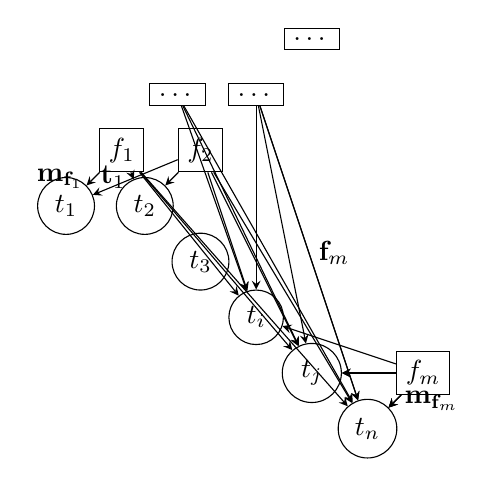
\begin{tikzpicture}[node distance=1cm, auto]
    % Place nodes
    \node[draw, circle] (t1) {$t_1$};
    \node[draw, circle] (t2) [right of=t1] {$t_2$};
    \node[draw, circle] (t3) [below right of=t2] {$t_3$};
    \node[draw, circle] (ti) [below right of=t3] {$t_i$};
    \node[draw, circle] (tj) [below right of=ti] {$t_j$};
    \node[draw, circle] (tn) [below right of=tj] {$t_n$};

    \node[draw, rectangle] (f1) [above right of=t1] {$f_{1}$};
    \node[draw, rectangle] (f2) [above right of=t2] {$f_{2}$};
    \node[draw, rectangle] (fm) [above right of=tn] {$f_{m}$};

    \node[draw, rectangle] (fmu) [above right of=f2] {$\dots$};
    \node[draw, rectangle] (fmi) [above right of=f1] {$\dots$};
    \node[draw, rectangle] (fmiu) [above right of=fmu] {$\dots$};

    % Draw edges
    \path[-stealth]
        (f1) edge node [left] {$\mathbf{m}_{\mathbf{f}_{1}}$} (t1)
        (f2) edge node [left] {$\mathbf{t}_1$} (t1)
        (f1) edge node [left] {} (t2)
        (f2) edge node [left] {} (t2)
        (fm) edge node [right] {$\mathbf{m}_{\mathbf{f}_{m}}$} (tn)
        (fmu) edge node [right] {$\mathbf{f}_{m}$} (tn)
        (fmu) edge node [left] {} (ti)
        (fmi) edge node [left] {} (ti)
        (f1) edge node [right] {} (ti)
        (f2) edge node [right] {} (ti)
        (fm) edge node [right] {} (ti)
        (fm) edge node [right] {} (tj)
        (fm) edge node [right] {} (tn)
        (fmu) edge node [right] {} (tj)
        (fmi) edge node [right] {} (tj)
        (f1) edge node [right] {} (tj)
        (f2) edge node [right] {} (tj)
        (fm) edge node [right] {} (tj)
        (fm) edge node [right] {} (tn)
        (fmu) edge node [right] {} (tn)
        (fmi) edge node [right] {} (tn)
        (f1) edge node [right] {} (tn)
        (f2) edge node [right] {} (tn);
\end{tikzpicture}

\end{document}